% Created by tikzDevice version 0.12.6 on 2026-02-22 21:43:33
% !TEX encoding = UTF-8 Unicode
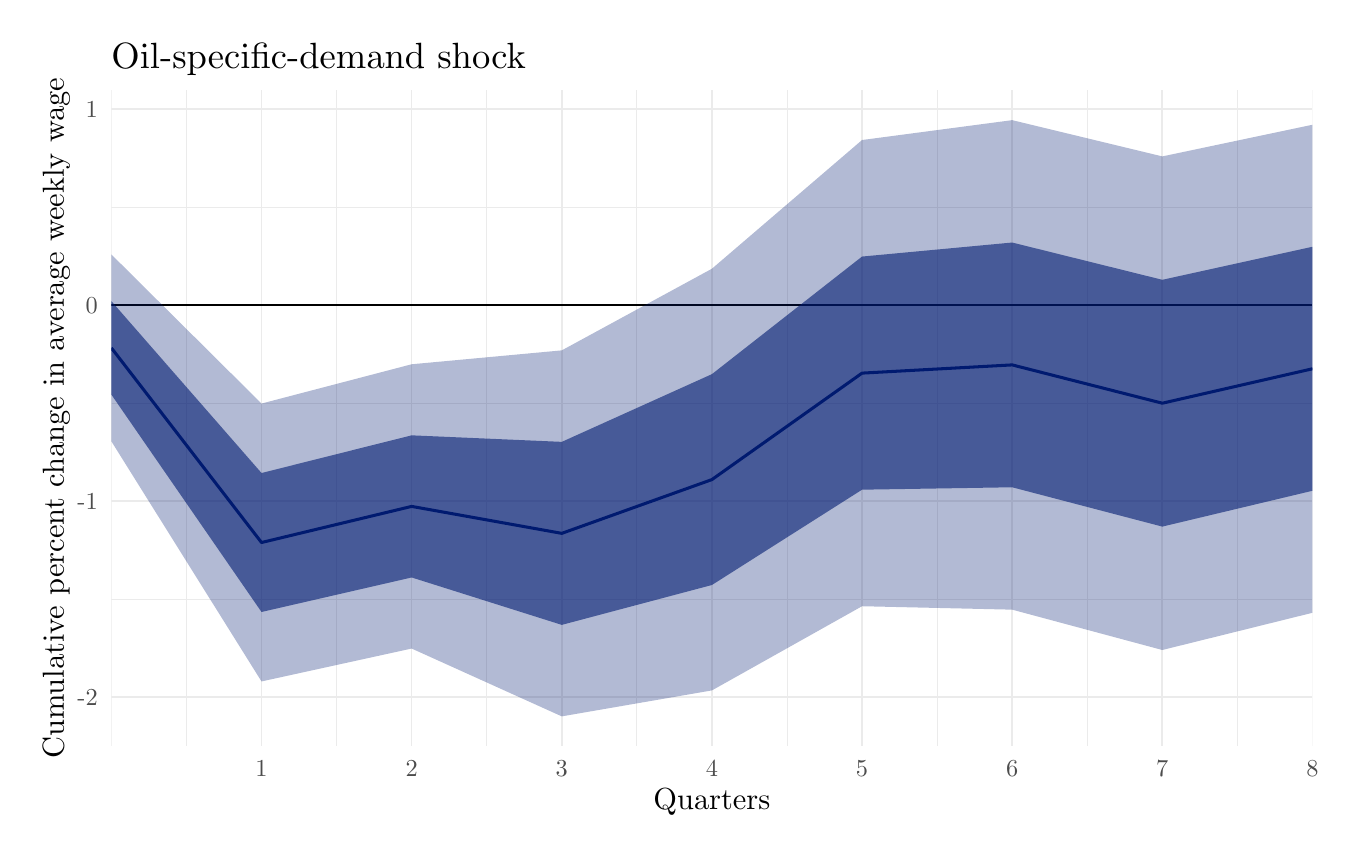
\begin{tikzpicture}[x=1pt,y=1pt]
\definecolor{fillColor}{RGB}{255,255,255}
\path[use as bounding box,fill=fillColor,fill opacity=0.00] (0,0) rectangle (469.75,290.32);
\begin{scope}
\path[clip] ( 30.25, 30.69) rectangle (464.26,267.67);
\definecolor{drawColor}{gray}{0.92}

\path[draw=drawColor,line width= 0.3pt,line join=round] ( 30.25, 83.86) --
	(464.26, 83.86);

\path[draw=drawColor,line width= 0.3pt,line join=round] ( 30.25,154.65) --
	(464.26,154.65);

\path[draw=drawColor,line width= 0.3pt,line join=round] ( 30.25,225.45) --
	(464.26,225.45);

\path[draw=drawColor,line width= 0.3pt,line join=round] ( 30.25, 30.69) --
	( 30.25,267.67);

\path[draw=drawColor,line width= 0.3pt,line join=round] ( 57.37, 30.69) --
	( 57.37,267.67);

\path[draw=drawColor,line width= 0.3pt,line join=round] (111.62, 30.69) --
	(111.62,267.67);

\path[draw=drawColor,line width= 0.3pt,line join=round] (165.87, 30.69) --
	(165.87,267.67);

\path[draw=drawColor,line width= 0.3pt,line join=round] (220.12, 30.69) --
	(220.12,267.67);

\path[draw=drawColor,line width= 0.3pt,line join=round] (274.38, 30.69) --
	(274.38,267.67);

\path[draw=drawColor,line width= 0.3pt,line join=round] (328.63, 30.69) --
	(328.63,267.67);

\path[draw=drawColor,line width= 0.3pt,line join=round] (382.88, 30.69) --
	(382.88,267.67);

\path[draw=drawColor,line width= 0.3pt,line join=round] (437.13, 30.69) --
	(437.13,267.67);

\path[draw=drawColor,line width= 0.6pt,line join=round] ( 30.25, 48.46) --
	(464.26, 48.46);

\path[draw=drawColor,line width= 0.6pt,line join=round] ( 30.25,119.26) --
	(464.26,119.26);

\path[draw=drawColor,line width= 0.6pt,line join=round] ( 30.25,190.05) --
	(464.26,190.05);

\path[draw=drawColor,line width= 0.6pt,line join=round] ( 30.25,260.85) --
	(464.26,260.85);

\path[draw=drawColor,line width= 0.6pt,line join=round] ( 84.50, 30.69) --
	( 84.50,267.67);

\path[draw=drawColor,line width= 0.6pt,line join=round] (138.75, 30.69) --
	(138.75,267.67);

\path[draw=drawColor,line width= 0.6pt,line join=round] (193.00, 30.69) --
	(193.00,267.67);

\path[draw=drawColor,line width= 0.6pt,line join=round] (247.25, 30.69) --
	(247.25,267.67);

\path[draw=drawColor,line width= 0.6pt,line join=round] (301.50, 30.69) --
	(301.50,267.67);

\path[draw=drawColor,line width= 0.6pt,line join=round] (355.75, 30.69) --
	(355.75,267.67);

\path[draw=drawColor,line width= 0.6pt,line join=round] (410.00, 30.69) --
	(410.00,267.67);

\path[draw=drawColor,line width= 0.6pt,line join=round] (464.26, 30.69) --
	(464.26,267.67);
\definecolor{drawColor}{RGB}{0,0,0}

\path[draw=drawColor,line width= 0.6pt,line join=round] ( 30.25,190.05) -- (464.26,190.05);
\definecolor{drawColor}{RGB}{0,26,112}

\path[draw=drawColor,line width= 1.1pt,line join=round] ( 30.25,174.60) --
	( 84.50,104.28) --
	(138.75,117.33) --
	(193.00,107.59) --
	(247.25,127.02) --
	(301.50,165.49) --
	(355.75,168.46) --
	(410.00,154.62) --
	(464.26,167.06);
\definecolor{fillColor}{RGB}{0,26,112}

\path[fill=fillColor,fill opacity=0.60] ( 30.25,191.49) --
	( 84.50,129.39) --
	(138.75,143.01) --
	(193.00,140.65) --
	(247.25,165.12) --
	(301.50,207.61) --
	(355.75,212.68) --
	(410.00,199.21) --
	(464.26,211.15) --
	(464.26,122.98) --
	(410.00,110.03) --
	(355.75,124.24) --
	(301.50,123.37) --
	(247.25, 88.93) --
	(193.00, 74.52) --
	(138.75, 91.65) --
	( 84.50, 79.18) --
	( 30.25,157.72) --
	cycle;

\path[] ( 30.25,191.49) --
	( 84.50,129.39) --
	(138.75,143.01) --
	(193.00,140.65) --
	(247.25,165.12) --
	(301.50,207.61) --
	(355.75,212.68) --
	(410.00,199.21) --
	(464.26,211.15);

\path[] (464.26,122.98) --
	(410.00,110.03) --
	(355.75,124.24) --
	(301.50,123.37) --
	(247.25, 88.93) --
	(193.00, 74.52) --
	(138.75, 91.65) --
	( 84.50, 79.18) --
	( 30.25,157.72);
\definecolor{fillColor}{RGB}{0,26,112}

\path[fill=fillColor,fill opacity=0.30] ( 30.25,208.37) --
	( 84.50,154.49) --
	(138.75,168.69) --
	(193.00,173.71) --
	(247.25,203.21) --
	(301.50,249.72) --
	(355.75,256.90) --
	(410.00,243.80) --
	(464.26,255.24) --
	(464.26, 78.89) --
	(410.00, 65.44) --
	(355.75, 80.02) --
	(301.50, 81.26) --
	(247.25, 50.84) --
	(193.00, 41.46) --
	(138.75, 65.97) --
	( 84.50, 54.08) --
	( 30.25,140.83) --
	cycle;

\path[] ( 30.25,208.37) --
	( 84.50,154.49) --
	(138.75,168.69) --
	(193.00,173.71) --
	(247.25,203.21) --
	(301.50,249.72) --
	(355.75,256.90) --
	(410.00,243.80) --
	(464.26,255.24);

\path[] (464.26, 78.89) --
	(410.00, 65.44) --
	(355.75, 80.02) --
	(301.50, 81.26) --
	(247.25, 50.84) --
	(193.00, 41.46) --
	(138.75, 65.97) --
	( 84.50, 54.08) --
	( 30.25,140.83);
\end{scope}
\begin{scope}
\path[clip] (  0.00,  0.00) rectangle (469.75,290.32);
\definecolor{drawColor}{gray}{0.30}

\node[text=drawColor,anchor=base east,inner sep=0pt, outer sep=0pt, scale=  0.88] at ( 25.30, 45.43) {-2};

\node[text=drawColor,anchor=base east,inner sep=0pt, outer sep=0pt, scale=  0.88] at ( 25.30,116.23) {-1};

\node[text=drawColor,anchor=base east,inner sep=0pt, outer sep=0pt, scale=  0.88] at ( 25.30,187.02) {0};

\node[text=drawColor,anchor=base east,inner sep=0pt, outer sep=0pt, scale=  0.88] at ( 25.30,257.82) {1};
\end{scope}
\begin{scope}
\path[clip] (  0.00,  0.00) rectangle (469.75,290.32);
\definecolor{drawColor}{gray}{0.30}

\node[text=drawColor,anchor=base,inner sep=0pt, outer sep=0pt, scale=  0.88] at ( 84.50, 19.68) {1};

\node[text=drawColor,anchor=base,inner sep=0pt, outer sep=0pt, scale=  0.88] at (138.75, 19.68) {2};

\node[text=drawColor,anchor=base,inner sep=0pt, outer sep=0pt, scale=  0.88] at (193.00, 19.68) {3};

\node[text=drawColor,anchor=base,inner sep=0pt, outer sep=0pt, scale=  0.88] at (247.25, 19.68) {4};

\node[text=drawColor,anchor=base,inner sep=0pt, outer sep=0pt, scale=  0.88] at (301.50, 19.68) {5};

\node[text=drawColor,anchor=base,inner sep=0pt, outer sep=0pt, scale=  0.88] at (355.75, 19.68) {6};

\node[text=drawColor,anchor=base,inner sep=0pt, outer sep=0pt, scale=  0.88] at (410.00, 19.68) {7};

\node[text=drawColor,anchor=base,inner sep=0pt, outer sep=0pt, scale=  0.88] at (464.26, 19.68) {8};
\end{scope}
\begin{scope}
\path[clip] (  0.00,  0.00) rectangle (469.75,290.32);
\definecolor{drawColor}{RGB}{0,0,0}

\node[text=drawColor,anchor=base,inner sep=0pt, outer sep=0pt, scale=  1.10] at (247.25,  7.64) {Quarters};
\end{scope}
\begin{scope}
\path[clip] (  0.00,  0.00) rectangle (469.75,290.32);
\definecolor{drawColor}{RGB}{0,0,0}

\node[text=drawColor,rotate= 90.00,anchor=base,inner sep=0pt, outer sep=0pt, scale=  1.10] at ( 13.08,149.18) {Cumulative percent change in average weekly wage};
\end{scope}
\begin{scope}
\path[clip] (  0.00,  0.00) rectangle (469.75,290.32);
\definecolor{drawColor}{RGB}{0,0,0}

\node[text=drawColor,anchor=base west,inner sep=0pt, outer sep=0pt, scale=  1.32] at ( 30.25,275.73) {Oil-specific-demand shock};
\end{scope}
\end{tikzpicture}
